\documentclass[pdf]{beamer}
\mode<presentation>{}
\usetheme{Dresden}
\usepackage{apalike}
\usepackage{graphicx}
\usepackage{movie15}
\usepackage{mwe,tikz}
\usepackage[percent]{overpic}
\beamertemplatenavigationsymbolsempty
%% preamble
\title{Modified Dispersive Wave Equations}
\usepackage{subcaption}
\author{Jordan Pitt, Stephen Roberts and Christopher Zoppou \\ Australian National University}
\newcommand\solidrule[1][0.25cm]{\rule[0.5ex]{#1}{1pt}}
\newcommand\dashedrule{\mbox{\solidrule[2mm]\hspace{2mm}\solidrule[2mm]}}
\newcommand{\dotrule}[1]{%
	\parbox[]{#1}{\dotfill}}

\setbeamertemplate{itemize item}[triangle]

\newcommand\T{\rule{0pt}{3ex }}       % Top table strut
\newcommand\B{\rule[-4ex]{0pt}{4ex }} % Bottom table strut

\begin{document}
	
\begin{frame}[plain]{}
\begin{tikzpicture}[remember picture,overlay]
\node[anchor=north east, inner sep=0pt] at (current page.north east) {
	\includemovie[
	poster,
	text={}
	]{\paperwidth}{\paperheight}{./Videos/Dambreak.avi}
};
\end{tikzpicture}
\end{frame}
	
	
%% title frame
\begin{frame}
\titlepage
\end{frame}
%% normal frame
	

%Do a brief show pictures of water waves, hazards posed
%Move onto the equations, with a picture
%Method: in terms of polynomial representation, FEM, FVM
%Validation: Present results of linear analysis: stability and dispersion analysis, then numerical solution comparisons

\begin{frame}{Outline}
	\begin{itemize}
		\item Motivation
		\item Equations
		\item Scheme
		\item Validation
	\end{itemize}
\end{frame}
\section{Motivation}
%Wave modelling
\begin{frame}{Motivation - Water Waves}
We require accurate models of water waves to understand natural hazards in particular
	\begin{itemize}
		\item Tsunamis
		\item Storm Surges
	\end{itemize}
\end{frame}

\begin{frame}{Motivation}
\begin{figure}
	\centering
	\begin{subfigure}{0.49\textwidth}
		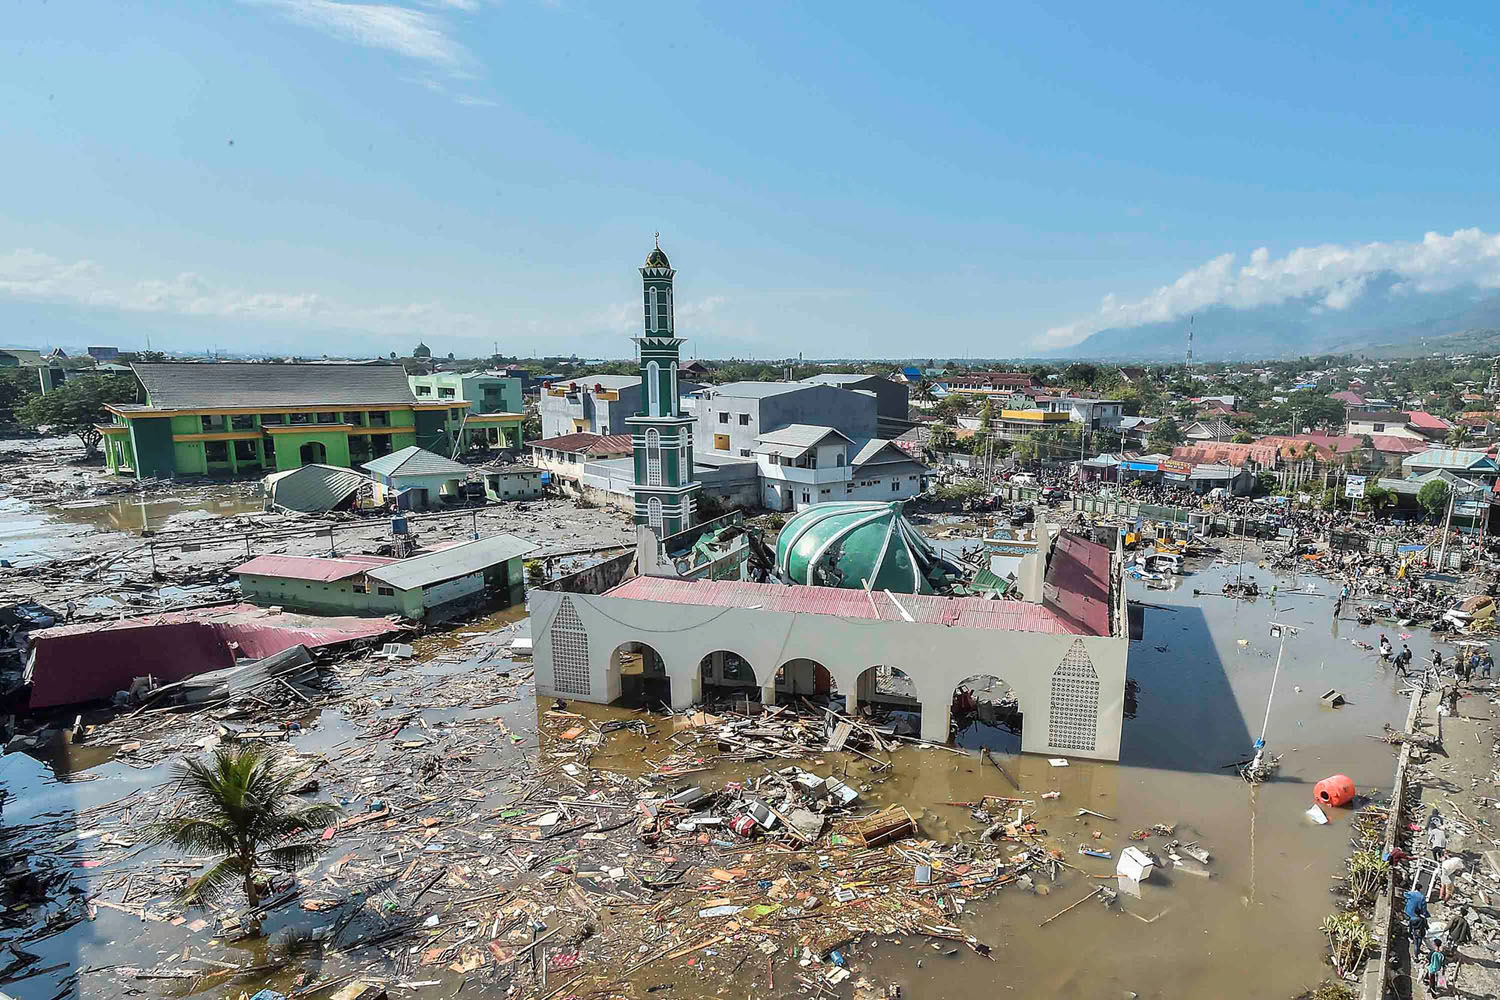
\includegraphics[width=0.9\textwidth]{./Pics/Web/SualwesiTsunami.jpg}
		\caption{Sulawesi Tsunami (Indonesia, 2018).}
	\end{subfigure}
	\begin{subfigure}{0.49\textwidth}
	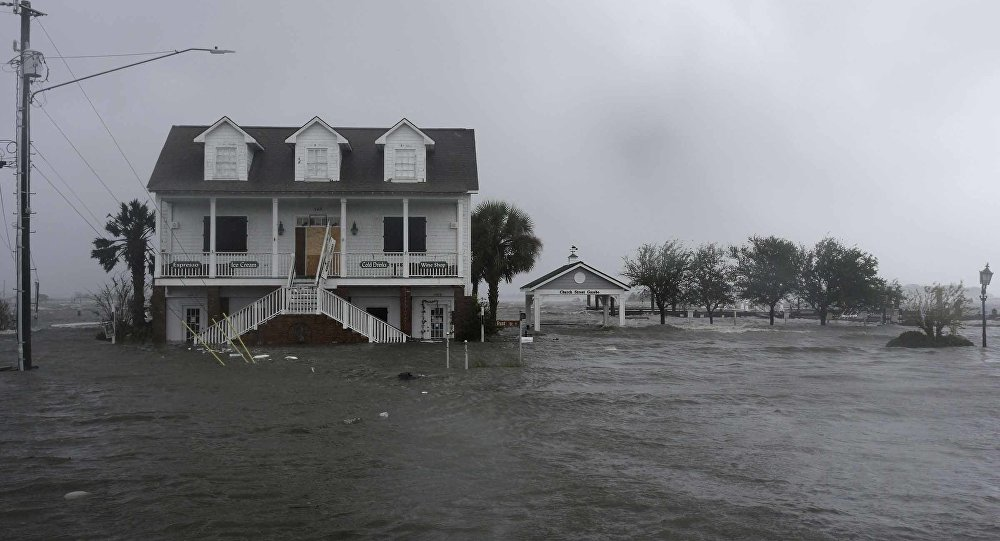
\includegraphics[width=1.1\textwidth]{./Pics/Web/HurricaneFlorence.jpg}
	\subcaption{Hurricane Florence (U.S.A, 2018)}
	\end{subfigure}
\end{figure}
\end{frame}

\begin{frame}{Motivation}
\begin{figure}
	\centering
	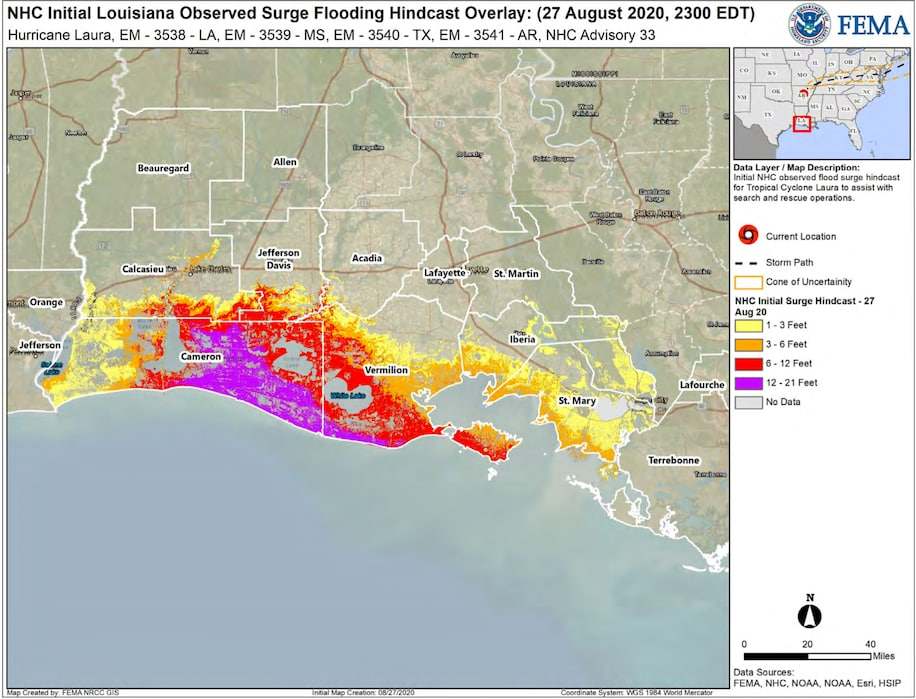
\includegraphics[width=0.7\textwidth]{./Pics/Web/StormSurgeLaura.jpeg}
	\caption{Hurricane Laura (U.S.A, 2020).}
\end{figure}
\end{frame}

\begin{frame}{Motivation - Water Waves}
We require accurate models of water waves to understand natural hazards in particular
\begin{itemize}
	\item Tsunamis
	\item Storm Surges
\end{itemize}
\bigskip
Current models built on models where wave speed independent of frequency (Shallow Water Wave Equations). 
\pause

\bigskip
What's the effect of wave frequency effects on these natural hazards?
\end{frame}

%Considering wave properties of small amplitude waves on a large background of still water
\begin{frame}{Dispersion Relationship of Water Waves (Linear Theory)}
\begin{figure}
	\centering
	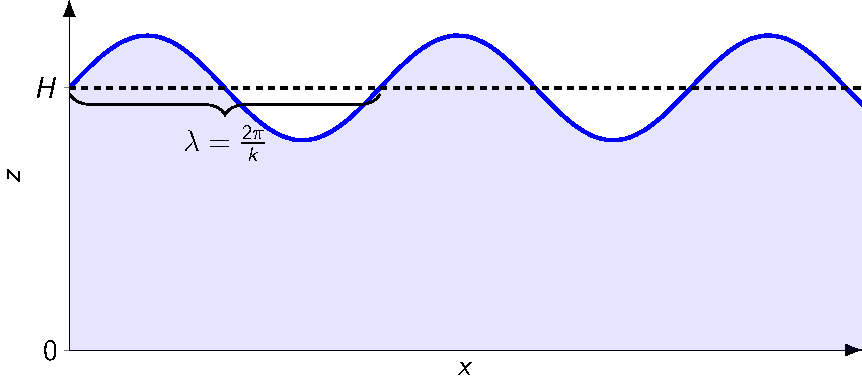
\includegraphics[width=0.9\textwidth]{./Pics/Tex/Explanatory/DispersionPlot/Dispersion.pdf}
\end{figure}
\end{frame}

\begin{frame}{Dispersion Relationship of Water Waves (Linear Theory)}
\begin{figure}
	\centering
	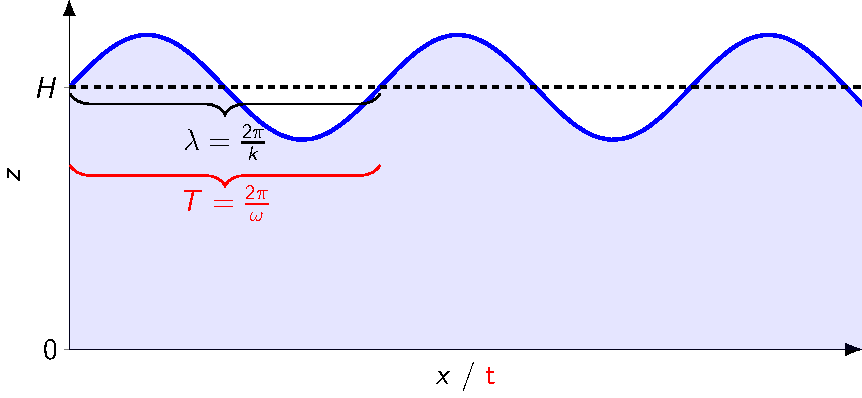
\includegraphics[width=0.9\textwidth]{./Pics/Tex/Explanatory/DispersionPlot/Dispersion_Analagous.pdf}
\end{figure}
\end{frame}

\begin{frame}{Dispersion Relationship of Water Waves (Linear Theory)}
\[\omega^2 = g k \tanh\left(kH\right) \]
Gives the angular frequency ($\omega$) as a function of gravitational acceleration ($g$), wave number ($k$) and mean background water depth ($H$). 

\bigskip
Phase speed ($c$)
\[c^2 = \frac{\omega^2}{k^2} = \frac{g}{k} \tanh\left(kH\right) \]
\end{frame}

\begin{frame}{Taylor Expansion of Phase Speed in $k$}
\[c^2  = \frac{g}{k} \tanh\left(kH\right) = gH - {\color{blue}\frac{1}{3} gH^3 k^2} + {\color{red}\frac{2}{15} g H^5 k^4} + \mathcal{O}\left(k^5\right) \]
\pause
Resulting non-linear equations
\begin{itemize}
	\item Non-dispersive Shallow Water Wave Equations
	\item \color{blue} Serre Equations
	\item \color{red} Improved Dispersion Serre Equations
\end{itemize}
Modified Dispersive Wave Equations generalise all these. 
\end{frame}


%To answer this effect we need a model
%This ones nice because it has conservation of mass, momentum and energy
%Allows the strength of dispersion to be altered to compare effect
% Why blue term? -
\section{Model}
\begin{frame}{Set Up}
Equations for conservation of mass and momentum written in terms of the water depth $h(x,t)$, the depth average horizontal velocity $u(x,t)$ and acceleration due to gravity $g$.
\begin{figure}
	\centering
	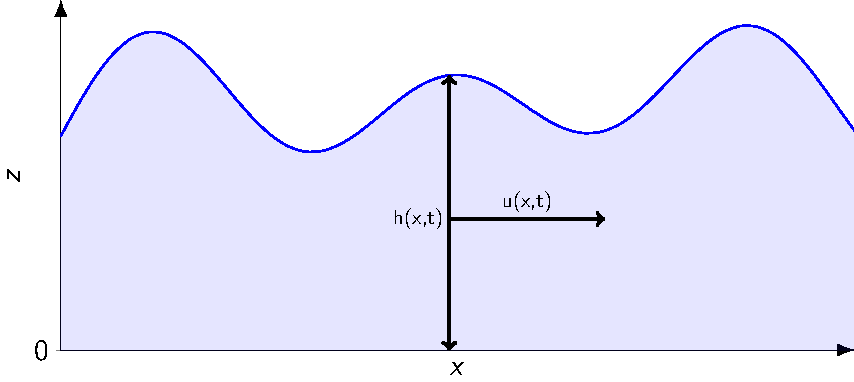
\includegraphics[width=0.9\textwidth]{./Pics/Tex/Explanatory/Setupplot/Waves.pdf}
	\caption{Relevant Quantities.}
\end{figure}
\end{frame}

%Only need blue term to get the relevant blue term in dispersion
%need both to get the red term
\begin{frame}{Modified Dispersive Wave Equations}
\begin{align*}
&\dfrac{\partial h}{\partial t} + \dfrac{\partial (hu)}{\partial x} = 0\\
&\dfrac{\partial (hu)}{\partial t} + \dfrac{\partial }{\partial x} \left( hu^2 + \frac{1}{2}gh^2  +  {\color{blue} \frac{1}{2}h^3\beta_1 \Phi } -   {\color{red} \frac{1}{2}gh^2 \beta_2 \Psi}  \right)= 0 \\
\end{align*}
where
\begin{align*}
\color{blue} \Phi  & \color{blue}= \frac{\partial u}{\partial x}\frac{\partial u}{\partial x} - \frac{\partial^2 u}{\partial x \partial t} - u\frac{\partial^2 u}{\partial x^2} \\
\color{red} \Psi & \color{red}= h \frac{\partial^2 h}{\partial x^2} + \frac{1}{2} \frac{\partial h}{\partial x}\frac{\partial h}{\partial x} 
\end{align*}
\end{frame}

\begin{frame}{Dispersion Relation of Linearised Equations}
\begin{align*}
c_{\text{model}}^2 & = gH \dfrac{\beta_2 H^2 k^2 + 2}{ \beta_1H^2 k^2 + 2}
\\& = gH - {\color{blue} \frac{\left(\beta_1 - \beta_2\right)}{2}gH^3 k^2} + {\color{red}\frac{\beta_1\left(\beta_1 - \beta_2\right)}{4} g H^5 k^4}  + \mathcal{O}\left(k^5\right)
\end{align*}
\end{frame}

\begin{frame}{Dispersion Relation of Linearised Equations}
\begin{align*}
c_{\text{model}}^2 & = gH \dfrac{\beta_2 H^2 k^2 + 2}{ \beta_1H^2 k^2 + 2}
\\& = gH - {\color{blue} \frac{\left(\beta_1 - \beta_2\right)}{2}gH^3 k^2} + {\color{red}\frac{\beta_1\left(\beta_1 - \beta_2\right)}{4} g H^5 k^4}  + \mathcal{O}\left(k^5\right) \\
\text{Want} \\c^2  &= \frac{g}{k} \tanh\left(kH\right) \\
 &= gH - {\color{blue}\frac{1}{3}g H^3 k^2} + {\color{red}\frac{2}{15} g H^5 k^4} + \mathcal{O}\left(k^5\right)
\end{align*}
\end{frame}

\begin{frame}{Dispersion Regions}
\begin{figure}
	\centering
	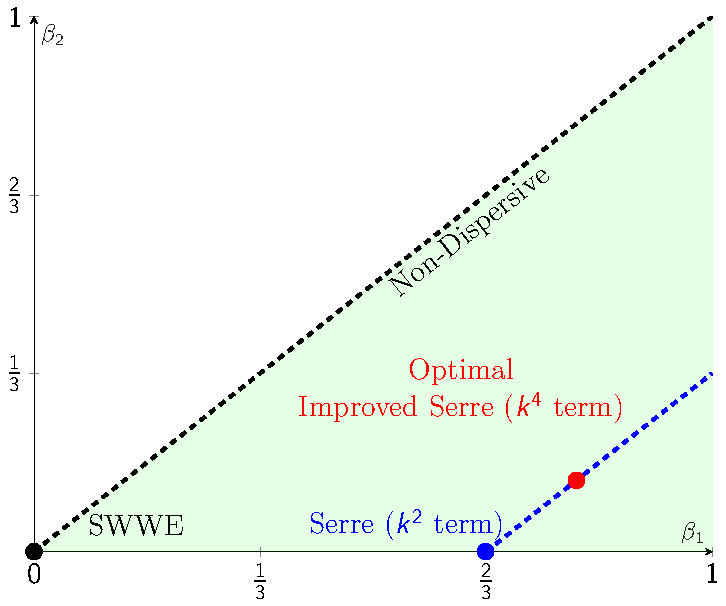
\includegraphics[width=0.7\textwidth]{./Pics/Tex/Explanatory/RegionsPlot/BetaPlotAll.pdf}
\end{figure}
\end{frame}

\begin{frame}{Dispersion Regions - First  Animation}
\begin{figure}
	\centering
	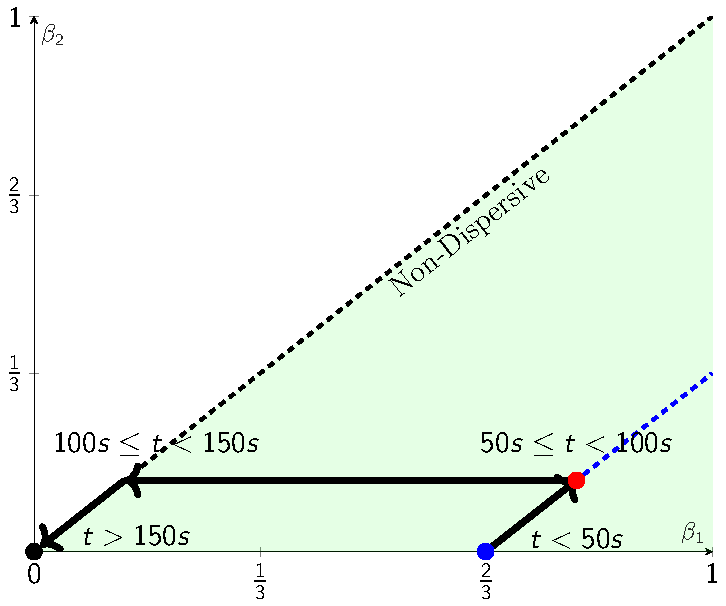
\includegraphics[width=0.7\textwidth]{./Pics/Tex/Explanatory/RegionsPlot/BetaPlotAllArrows.pdf}
\end{figure}
\end{frame}

\begin{frame}[plain]{}
\begin{tikzpicture}[remember picture,overlay]
\node[anchor=north east, inner sep=0pt] at (current page.north east) {
\includemovie[
poster,
text={}
]{\paperwidth}{\paperheight}{./Videos/Dambreak.avi}
 	};
\end{tikzpicture}
\end{frame}



\begin{frame}{Model - Conclusion}
\begin{itemize}
	\item We now have one set of equations we can solve that includes
	\begin{itemize}
		\item Non-dispersive wave models
		\item $k^2$ accurate dispersive wave models
		\item $k^4$ accurate dispersive wave models
	\end{itemize}
\end{itemize}
We can thus implement one numerical scheme and investigate the impact of different $\beta$ values to investigate effect of dispersion on natural hazards. 
\end{frame}


\section{Scheme}
%Dfficult to solve in primitive conservation law form because of mixed derivative
\begin{frame}{Equations}
\begin{align*}
&\dfrac{\partial h}{\partial t} + \dfrac{\partial (hu)}{\partial x} = 0\\
&\dfrac{\partial (hu)}{\partial t} + \dfrac{\partial }{\partial x} \left( hu^2 + \frac{1}{2}gh^2  +  {\color{blue} \frac{h^3}{2}\beta_1 \Phi } -   {\color{red} \frac{gh^2}{2} \beta_2 \Psi}  \right)= 0 \\
\end{align*}
where
\begin{align*}
\color{blue} \Phi  & \color{blue}= \frac{\partial u}{\partial x}\frac{\partial u}{\partial x} - \frac{\partial^2 u}{\partial x \partial t} - u\frac{\partial^2 u}{\partial x^2} \\
\color{red} \Psi & \color{red}= h \frac{\partial^2 h}{\partial x^2} + \frac{1}{2} \frac{\partial h}{\partial x}\frac{\partial h}{\partial x} 
\end{align*}
\end{frame}

%Can reformulate into conservative form
\begin{frame}{Reformulation}
\begin{align*}
&\dfrac{\partial h}{\partial t} + \dfrac{\partial (hu)}{\partial x} = 0\\
&\dfrac{\partial {\color{blue} G} }{\partial t}  + \dfrac{\partial}{\partial x} \Bigg( u{\color{blue} G} + \dfrac{gh^2}{2} - {\color{blue} \beta_1 h^3\dfrac{\partial u}{\partial x}\dfrac{\partial u}{\partial x} } \\ &- {\color{red}\frac{1}{2} \beta_2 g h^2  \left[h\frac{\partial^2 h}{\partial x^2} +   \frac{1}{2}\frac{\partial h}{\partial x}\frac{\partial h}{\partial x}\right] } \Bigg) = 0.
\end{align*}
where
\begin{gather*}
{\color{blue} G} = uh {\color{blue} - \frac{1}{2} \beta_1\dfrac{\partial }{\partial x} \left ( h^3 \dfrac{\partial u}{\partial x} \right )}.
\end{gather*}
\end{frame}


\begin{frame}{Central Idea - Starting with $h$ and $G$}
Solve
\begin{gather*}
{\color{blue} G} = uh {\color{blue} - \frac{1}{2} \beta_1\dfrac{\partial }{\partial x} \left ( h^3 \dfrac{\partial u}{\partial x} \right )}.
\end{gather*}
to obtain $u$.

\bigskip
\pause
Then solve
\begin{align*}
&\dfrac{\partial h}{\partial t} + \dfrac{\partial (hu)}{\partial x} = 0\\
&\dfrac{\partial {\color{blue} G} }{\partial t}  + \dfrac{\partial}{\partial x} \Bigg( u{\color{blue} G} + \dfrac{gh^2}{2} - {\color{blue} \beta_1 h^3\dfrac{\partial u}{\partial x}\dfrac{\partial u}{\partial x} } \\ &- {\color{red}\frac{1}{2} \beta_2 g h^2  \left[h\frac{\partial^2 h}{\partial x^2} +   \frac{1}{2}\frac{\partial h}{\partial x}\frac{\partial h}{\partial x}\right] } \Bigg) = 0.
\end{align*}
with a finite volume method to update $h$ and $G$ to next time. 
\end{frame}

\begin{frame}{First Example - Extension of Previous Methods for Serre}
\begin{itemize}
	\item Solve $u$ given $h$ and $G$, using a second-order finite difference approximation.
	\item Update $h$ and $G$ using a second-order finite volume approximation.
\end{itemize}
\end{frame}

\begin{frame}{Why Finite Volume?}
The central reason is robustness.
\begin{itemize}
	\item Equations possess weak solutions with discontinuities 
	\begin{itemize}
	\item Shallow Water Wave Equations (Shocks - Jump Discontinuity)
	\item Certain Parameter Combinations (Weak Discontinuities - Continuous with discontinuous derivative)
	\end{itemize}
	\item Reproduction of those underlying conservation properties.
\end{itemize}
We were able to produce the first well validated method this way. 
\end{frame}


\section{Validation}
\begin{frame}{Validation}
Analytic solutions only known for some $\beta$ values. 

\bigskip
Just $k^2$ accurate Serre today.
\end{frame}

\begin{frame}{
	Serre ($k^2$ accurate) Analytic Solution \hfill \hfill \hfill \hfill 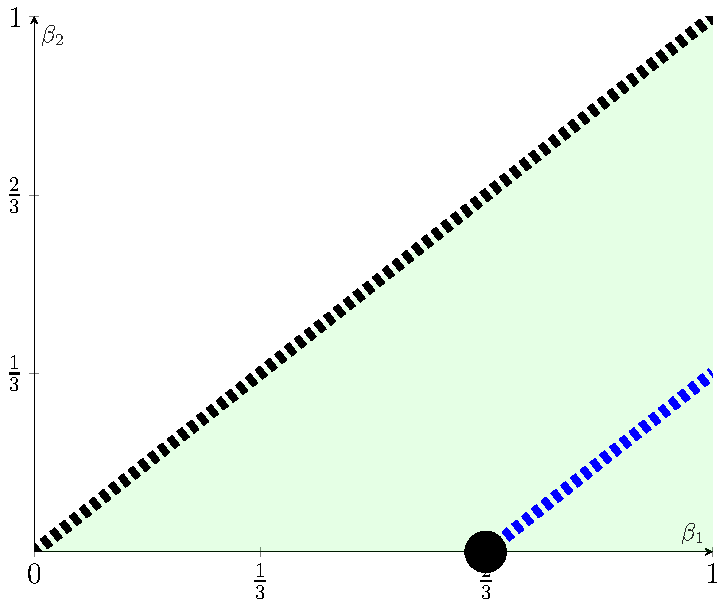
\includegraphics[width=2cm]{./Pics/Tex/Explanatory/MiniRegions/Serre.pdf}}
\begin{figure}
	\centering

	\includemovie[
	poster,
	text={}
	]{0.4\paperwidth}{0.4\paperheight}{./Videos/Soliton.avi}
\end{figure}
\end{frame}


\begin{frame}{
	Serre ($k^2$ accurate) Error \hfill \hfill \hfill \hfill 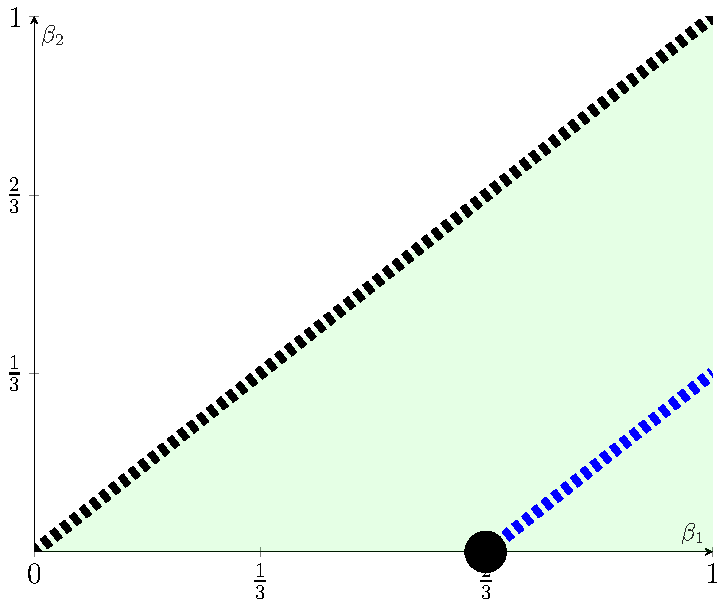
\includegraphics[width=2cm]{./Pics/Tex/Explanatory/MiniRegions/Serre.pdf}}
\begin{figure}
	\centering
	\begin{subfigure}{0.49\textwidth}
		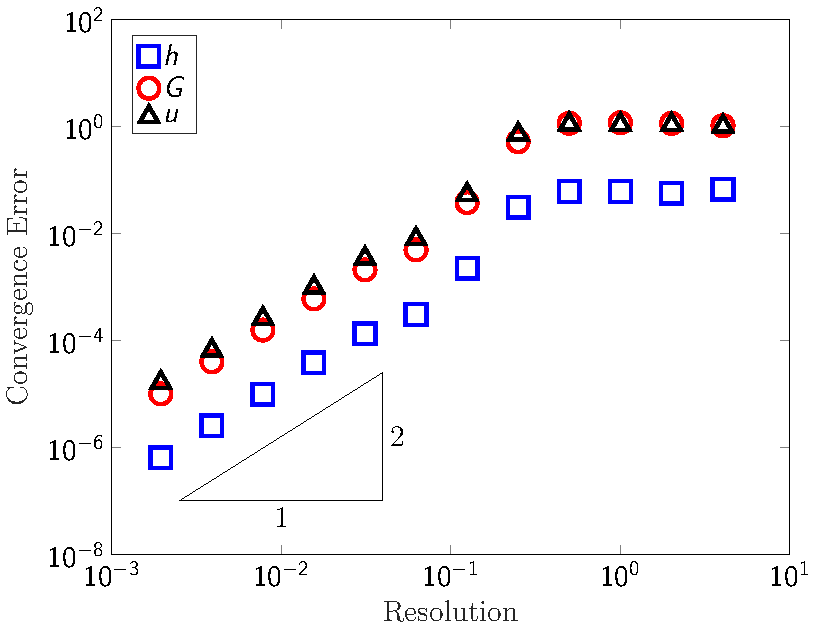
\includegraphics[width=0.9\textwidth]{./Pics/Tex/Results/Validation/Soliton/Convergence.pdf}
	\end{subfigure}
	\begin{subfigure}{0.49\textwidth}
		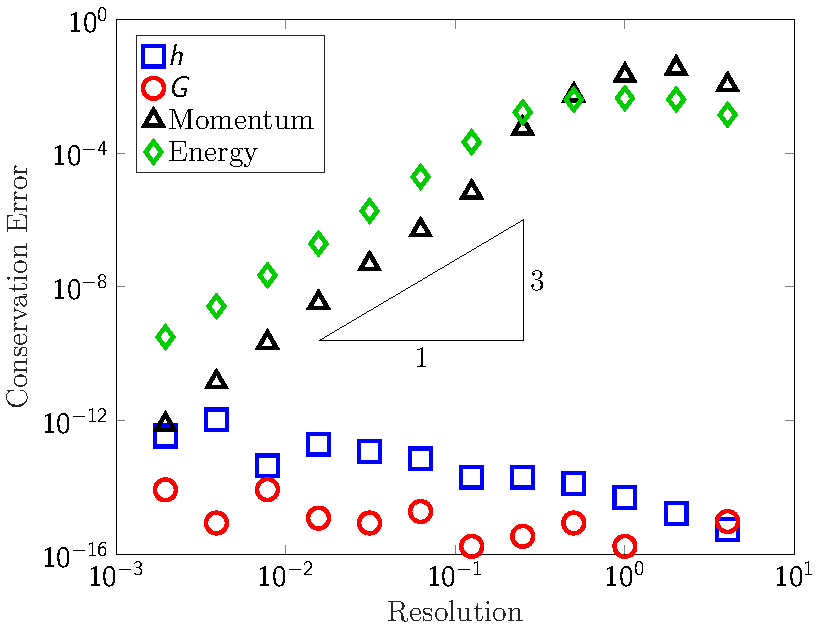
\includegraphics[width=0.9\textwidth]{./Pics/Tex/Results/Validation/Soliton/Conservation.pdf}
	\end{subfigure}
\end{figure}
\end{frame}


\begin{frame}{Conclusions}
\begin{itemize}
	\item Can solve these equations with our scheme
	\item First well validated robust method
\end{itemize}
Good progress towards addressing the motivation. 
\end{frame}


\begin{frame}
Thanks!
\end{frame}


\end{document}